
\begin{figure}
\centering
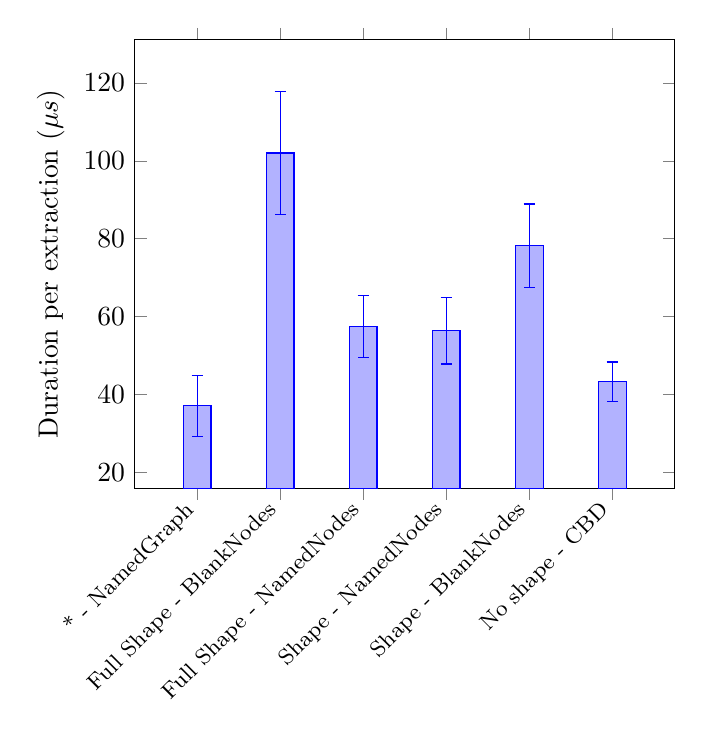
\begin{tikzpicture}
        \begin{axis}[
            ybar,
            enlargelimits=0.15,
            legend style={at={(0.5,-0.15)},
            anchor=north,legend columns=-1},
            ylabel={Duration per extraction ($\mu s$)},
            symbolic x coords={
* - NamedGraph,
Full Shape - BlankNodes,
Full Shape - NamedNodes,
Shape - NamedNodes,
Shape - BlankNodes,
No shape - CBD
            },
            xtick=data,
            x tick label style={font=\footnotesize,rotate=45, anchor=east},
            nodes near coords align={horizontal},
        ]
            \addplot+[
                error bars/.cd,
                y dir=both,
                y explicit
            ] coordinates {
         (* - NamedGraph, 37.1175404814876) +- (0, 7.848091109799674)
         (Full Shape - BlankNodes, 102.00427880882357) +- (0, 15.804602720751047)
         (Full Shape - NamedNodes, 57.47719474228394) +- (0, 8.05663661519078)
         (Shape - NamedNodes, 56.419020486111094) +- (0, 8.573803086683053)
         (Shape - BlankNodes, 78.15333630597017) +- (0, 10.75845180571196)
         (No shape - CBD, 43.26234066338073) +- (0, 5.098359156055337)

             };
        \end{axis}
    \end{tikzpicture}
    \caption{Graph depicting performance of inband extraction algorithm}
\end{figure}
